\section{Evaluation}

In this section, we will evaluate our solution and implementation in terms of security and performance. 

\subsection{Security Analysis}

Our adversarial model is that we assume the adversary has the capability to upload malicious logic to the PLC that will generate erroneous outputs or further compromise the entire PLC. After the entire PLC is compromised, we assume the attacker can even get access to the encryption key, which will be used to encrypt the next event, together with the encrypted logs that have not been sent to the server yet. This is a very strong adversarial model for a remote attacker who is connected over the network. Only when our solution is applied to a modern PLC or OpenPLC, meaning that the PLC logic and the   When our solution is applied to the legacy PLCs, the logging mechanism is implemented outside of the legacy PLCs as another hardware layer, so a remote attacker has no way to get the key in it.  

In addition, we assume that the logging mechanism is working properly until a certain point after the compromise initiates. In other words, we assume there exist a time window that the attacker has initiated the intrusion, but the logging is still working properly. The overall timeline can be illustrated as Figure.~\ref{fig:timeline}. 

\begin{figure*}[h]
  \centering
    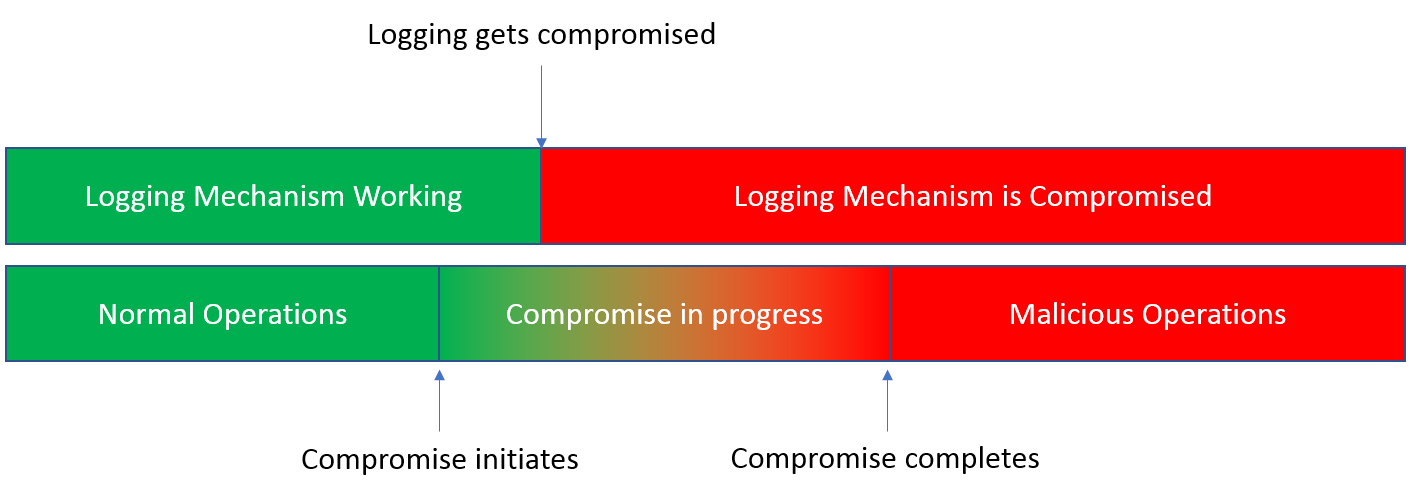
\includegraphics[width=\textwidth]{figs/timeline}
    \caption{Time line of one compromise.}
    \label{fig:timeline}
\end{figure*}

The time window between the start of a compromise and the moment that the logging failed is very critical. Essentially the logs generated in this time window tells the server that an intrusion is happening. The attacker has four different approaches to deal with this log, and all of them will lead to detection. We list all the four possible approaches below:

\begin{enumerate}
\item \textbf{Let the encrypted logs send to the server. } Since this log contains the information about intrusion, the adversary will be detected.

\item \textbf{Try to decrypt the logs.} Notice that, it is possible that the adversary compromises the device completely (i.e. knowing the current encryption key) before the log has been sent. But the previous log has already been encrypted and buffered, and the encryption key is updated in a forward secure way. The attacker has no chance to inverse the hash function and gets to know the previous encryption key. Therefore, the attacker is not able to decrypt the log, and has to send this log as it is. 

\item \textbf{Tamper with the encrypted logs.} The attacker can either send something random or replay a previous log about a clean state. Since the encryption key is updated after each event, the server with an updated key will not be able to decrypt this tampered log. Therefore, the server will also conclude that an intrusion is happening on this PLC. 

\item \textbf{Block the communication between the PLC and the server.} If the communication between the compromised PLC and the server is blocked, no log will arrive the server on time. Since the PLC is required to send the report periodically, any PLC which fails to send the log on time will be considered as compromised. 

\end{enumerate}     

To summarize, there is no way for the attackers to avoid detecting by our intrusion detection scheme. 

\subsection{Sensitivity of Detection}

Since our solution requires the logs from PLCs to be sent periodically, it is possible for the server to have a detection latency no larger than a reporting period. Hence, when we select the parameter of reporting period, we need to consider this detection latency as well. 
   
\subsection{Performance Overhead}